\subsection{Data Gatherer}\label{sec:impl-data-gatherer}
The data gatherer tool has been split into a number of files for readability and maintenance. Additionally significant portion of the code written has been tested with automated tests. Project structure is initially split between source code and test code folders, named \texttt{src} and \texttt{test} respectively. In each a number of resource files have been defined to support the program execution, mock server responses and data or provide additional information. .


\begin{figure}[!h]
    \centering
    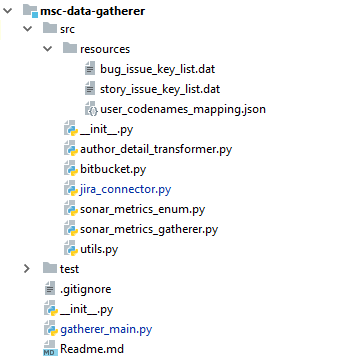
\includegraphics{Figures/impl_src_folder_files.png}
    \caption{Source Files Structure}
    \label{fig:impl-data-gatherer-source-files}
\end{figure}

Source folder structure has been illustrated in Figure \ref{fig:impl-data-gatherer-source-files} and it is comprised of the following elements:
\begin{enumerate}
    \item \texttt{gatherer\_main.py} - included in full in code excerpt \ref{code:gatherer_main.py}. Coordinates all data gathering operations. 
    \item\label{lst:impl.item:jira} \texttt{jira\_connector.py} - Handles all communication and authentication with a given JIRA server. From a list of JIRA keys contained in \texttt{bug\_issue\_key\_list.dat} and \texttt{story\_issue\_key\_list.dat} interrogates the server over REST API to obtain an ID attribute for each ticket. Then, again using JIRA's REST API, obtains a list of commits for a given JIRA ID for all code repositories. 
    
    At this step a number of infrastructure repositories that are maintenance only, or ones that are written in languages not supported by Sonar server, thus making it impossible to obtain code quality metrics, have been removed.
    
    In the next step all merge commits are being removed from the analysis as it would otherwise create duplicate data points. For detailed explanation refer to Section \ref{sec:design}. Additionally a number of files are removed from the analysis - for details on what file extensions were ignored as well as a brief reasoning for same, refer to Table \ref{tbl:file-extensions-excluded-from-analysis}.
    
    In the final step a list of initial metrics identifying a given commit is compiled. Alongside it, a map containing \texttt{issue\_key}, \texttt{source\_repository}, \texttt{commitId}, \texttt{path} and \texttt{repo\_code}, which is a unique 3-4 character abbreviation identifying a repository, is composed. Complete map containing both commit details as well as information necessary in the subsequent step is returned back to the coordinator file. 
    
    For code listing for this step refer to code excerpt \ref{code:jira-connector.py}
    
    \item\label{lst:impl.item:bitbucket} \texttt{bitbucket.py} - handles all communication and authentication with a given Bitbucket server. Given data provided by JIRA server from above item interrogates a specified Bitbucket server over REST API in order to obtain details of previous commit such as author and timestamp. As previously described in Section \ref{sec:design}, List \ref{lst:design:info-from-bitbucket} those details will be used in subsequent analysis steps to provide indication of developers' level of experience based on seniority as well as familiarity with a given product based on the amount of time spend on the project.
    
    Once all those details have been obtained an compiled they are returned to the coordinator file.
    Complete code listing is available from code excerpt \ref{code:bitbucket.py}.
    
    \item\label{lst:impl.item:sonar-metrics-gatherer} \texttt{sonar\_metrics\_gatherer.py} - is responsible for all communication via REST API with Sonar server instance. Using data gathered by JIRA and Bitbucket steps above it contacts Sonar server for each and every file, for each and every commit under each JIRA ticket and retrieves a specified list of code quality metrics. The list is defined in \texttt{sonar\_metrics\_enum.py} and it is comprehensive. 
    
    In order to retrieve code quality metrics first the expected parameters need to generated from data retrieved from both JIRA and Bitbucket - the expected data is called project component  and it is an unique identifier on Sonar Server for each file ever analyzed. The project component is in different format for some projects therefore it was necessary to model a number of generation use cases, as outlined in the \texttt{sonar\_component\_name\_generator} method in \ref{code:sonar-gatherer.py} code listing.
    
    One thing to note is that for different source code languages different metrics, especially with regards to the code coverage metrics can be provided by Sonar. For example for JavaScript based languages such as Angular JS there is a separate position for integration, or IT, coverage, whereas for Java and other JVM based languages that metric is rarely provided. In JVM based languages it has been folded into the \texttt{overall code coverage} metric instead.
    
    \item\label{lst:impl.item:author-encoder} \texttt{author\_detail\_transformer.py} is responsible for encoding authors' full names into code names to obfuscate sensitive identity details. it is invoked after code quality metrics have been gathered by \texttt{SonarMetricsGatherer} class.
    
\end{enumerate}
Once all metrics have been gathered and encoded they are combined with data gathered in previous steps and all information is output into a \texttt{results.csv} file representing complete dataset to be analyzed. For code listing for this step refer to code excerpt \ref{code:sonar-gatherer.py}.

\begin{table}[h!]
\centering
\caption{Files excluded from the analysis by extension or suffix}
\label{tbl:file-extensions-excluded-from-analysis}
\begin{tabular}{@{}llll@{}}
\toprule
\multicolumn{4}{c}{Exclusion Patterns} \\ \midrule
.*Test.*.java & .*Interface.*\textbackslash{}.java & .*NameToIndex\textbackslash{}.java & .*\textbackslash{}.jar \\
.*Test.*.kt & .*Interface.*\textbackslash{}.kt & .*Config.kt & .*Dto.*kt \\
.*\textbackslash{}.e2e-spec.js & .*\textbackslash{}.stub.js & .*\textbackslash{}.po.js & .*spec.js \\
.*\textbackslash{}.ico & .*\textbackslash{}.npmrc & .*\textbackslash{}.conf.js & .*gulpfile.js \\
.*ColumnDef.js & .*Spec.js & .*Decorator.js & \textbackslash{}.eslintrc \\
.*\textbackslash{}.gitattributes & .*\textbackslash{}.sql & .*\textbackslash{}.csv & .*\textbackslash{}.xlsx \\
.*\textbackslash{}.txt & .*\textbackslash{}.xlsm & .*\textbackslash{}.yaml & .*\textbackslash{}.yml \\
.*WriteService.* & .*DeleteService.* & .*CreateService.* & .*\textbackslash{}.lock \\
.*.gradle & .*\textbackslash{}.?factory.js & .*\textbackslash{}.css & .*.config.js \\
.*Config.java & .*\textbackslash{}.html & .*\textbackslash{}.svg & .*ColumnDefs.js \\
.*\textbackslash{}.gz & .*ReadService.* & \textbackslash{}.gitignore & .*\textbackslash{}.json \\
.*\textbackslash{}.war & .*Enum.*kt & .*\textbackslash{}.scss & .*factories.js \\
.*Jenkinsfile.* & .*\textbackslash{}.xml & .*\textbackslash{}.md & .*\textbackslash{}.properties \\ \bottomrule
\end{tabular}
\end{table}




\begin{landscape}

\begin{code}
\captionof{listing}{Main data gathering component - the coordinator}
\label{code:gatherer_main.py}
\begin{minted}[breaklines]{python}
class Gatherer:

    def __init__(self):
        self.header_printed = False

    def main(self, username, password, jira_keys, is_bug_file):
        for jira_key in jira_keys:
            jira_obj = JiraConnector(username, password)
            # get metrics from JIRA
            files, commit_details = jira_obj.main(jira_key)

            sonar_obj = SonarMetricsGatherer(username, password)
            output = []
            bb = Bitbucket(username, password)
            # get information about previous commits
            prev_commit_details = bb.get_prev_commit_details_per_filepath(commit_details)
            # encode author's fullname for identity protection
            prev_commit_details = AuthorDetailsTransformer().transform_names_into_codenames(prev_commit_details)

            for file in files.keys():
                repo_file_is_in = files[file]
                component_key = sonar_obj.get_project_key_by_project_name(repo_file_is_in)

                # check if component key was generated correctly
                if len(component_key) <= 0:
                    self.log_jira_error(jira_key)
                    continue

                # get component_name
                component_name = sonar_obj.sonar_component_name_generator(component_key, file)
               
                # check if component name was generated correctly
                if len(component_name) <= 0:
                    self.log_jira_error(jira_key)
                    continue

                sorted_metrics_dict = sonar_obj.main(component_name, repo_file_is_in)
               
                # check if metrics were generated correctly
                if len(sorted_metrics_dict) > 0:
                    sorted_metrics_dict['source_repo'] = repo_file_is_in
                    sorted_metrics_dict['is_bug'] = is_bug_file
                    sorted_metrics_dict['issue_key'] = jira_key
                    combined = sorted_metrics_dict.copy()
                    combined.update(prev_commit_details[file])
                    output.append(combined)

                    sonar_obj.save_to_csv(header_printed=self.header_printed, list_of_metric_dicts=output,
                                          out_path='results.csv')
                    self.header_printed = True  # ensure that header is only appended once to target CSV
                else:
                    self.log_jira_error(jira_key)

    def log_jira_error(self, jira_key):
        print('Error with processing JIRA: {0}'.format(jira_key))

    def load_jira_key_files(self, file_location):
        values = []
        with open(file_location) as f:
            for line in f:
                line = line.replace('\n', '')
                values.append(line)
        return values


if __name__ == '__main__':
    start_time = time.time()
    urllib3.disable_warnings()
    username = None
    password = None
    if len(sys.argv) > 2:
        username = sys.argv[1]
        password = sys.argv[2]
    try:
        obj = Gatherer()
        # get data from bug tickets
        jira_keys = obj.load_jira_key_files('src/resources/bug_issue_key_list.dat')
        obj.main(username, password, jira_keys, True)

        # get data from regular tickets
        jira_keys = obj.load_jira_key_files('src/resources/story_issue_key_list.dat')
        obj.main(username, password, jira_keys, False)
        print('Operation duration: {0}'.format(time.time() - start_time))
    except Exception as e:
        print('Operation completed with an error. Duration: {0}'.format(time.time() - start_time))

\end{minted}
\end{code}



\begin{code}
\captionof{listing}{JIRA Connector - extracts relevant metrics from a given JIRA ticket}
\label{code:jira-connector.py}
\begin{minted}[breaklines]{python}
class JiraConnector:
    server_url_base = 'https://cksvnprd01.corp.emc.com/jira'
    url = 'https://cksvnprd01.corp.emc.com/jira/rest/webResources/1.0/resources'

    username = ''
    password = ''

    def __init__(self, username, password):
        self.username = username
        self.password = password

    def main(self, issue_key='ZZZ-1234'):
        issue_id = self.get_jira_id_from_jira_key(issue_key)

        resp = self.get_commit_details_for_a_jira_id(issue_id)
        return self.get_filenames_from_commits(resp)

    def is_valid_project(self, project_name):
        exclusions_pattern = '' # omitted for brevity
        exclusions_re = re.compile(exclusions_pattern)

        if exclusions_re.match(project_name):
            return False
        else:
            return True

    def get_jira_details_url(self, key):
        base_url = self.server_url_base + '/rest/api/2/issue/{0}'
        return base_url.format(key)

    def get_jira_id_from_jira_details(self, jira_details):
        id_key = 'id'
        return jira_details.get(id_key)

    def get_jira_id_from_jira_key(self, jira_key):
        url = self.get_jira_details_url(jira_key)

        jira_details_resp = requests.get(url, auth=HTTPBasicAuth(self.username, self.password), verify=False)
        if (jira_details_resp.status_code == 404):
            backup_url = 'https://cksvnprd01.corp.emc.com:4443/joanna/rest/api/2/issue/{0}'.format(jira_key)
            jira_details_resp = requests.get(backup_url, auth=HTTPBasicAuth(self.username, self.password), verify=False)
            print(backup_url)
            print(jira_details_resp.text)
        return self.get_jira_id_from_jira_details(jira_details_resp.json())


    def get_commit_details_for_a_jira_id(self, jira_id):
        resp = requests.get(self.get_commit_details_url(jira_id), auth=HTTPBasicAuth(self.username, self.password),
                            verify=False)
        return resp.json()

    def get_commit_details_url(self, id):
        url_base = self.server_url_base + '/rest/dev-status/1.0/issue/detail?issueId={0}&applicationType=stash&dataType=repository&_=1549641890823'
        return url_base.format(id)

    def get_repositories_from_json_response(self, json_details):
        repositories_section = json_details['detail'][0]['repositories']
        return repositories_section

    def get_repo_slug_from_repo_url(self, repo_url):
        slug_expr = re.compile('http.?://gssd-stash.isus.emc.com/projects/(\w+)\/.*')
        return slug_expr.match(repo_url).group(1)

    def get_commits_from_json_response(self, input_json):
        repositories_section = self.get_repositories_from_json_response(input_json)

        commits_in_repo = {}
        for repo in repositories_section:
            repo_name = repo['name']
            if self.is_valid_project(repo_name):
                repo_slug = self.get_repo_slug_from_repo_url(repo['url'])
                for commit in repo['commits']:
                    if commit['merge'] is False:

                        commit['repo_slug'] = repo_slug
                        if repo_name not in commits_in_repo.keys():
                            current_commits = [commit]
                            commits_in_repo[repo_name] = []
                            commits_in_repo[repo_name] = current_commits
                        else:
                            current_commits = commits_in_repo[repo_name]
                            current_commits.append(commit)
                            commits_in_repo[repo_name] = current_commits
        return commits_in_repo

    def get_filenames_from_commits(self, json):
        repo_to_commits_dict = self.get_commits_from_json_response(json)
        filenames = {}
        commit_details = {}
        java_exclusions = '' # omitted for clarity
        kotlin_exclusions = '' # omitted for clarity
        javascript_exclusions = '' # omitted for clarity
        other_exclusions = '' # omitted for clarity
        java_re = re.compile(java_exclusions)
        kotlin_re = re.compile(kotlin_exclusions)
        javascript_re = re.compile(javascript_exclusions)
        other_re = re.compile(other_exclusions)
        for repo in repo_to_commits_dict.keys():
            for commit in repo_to_commits_dict[repo]:
                for file in commit['files']:
                    if java_re.match(file['path']) or kotlin_re.match(file['path']) or javascript_re.match(
                            file['path']) or other_re.match(file['path']):
                        pass
                    else:
                        filenames[file['path']] = repo
                        commit_id = commit['id']
                        repo_slug = commit['repo_slug']
                        partial = {}
                        partial['commitId'] = commit_id
                        partial['target_repo'] = repo
                        partial['repo_code'] = repo_slug
                        commit_details[file['path']] = partial
        return filenames, commit_details

    def get_repo_name(self, json):
        return self.get_repositories_from_json_response(json)[0]['name']
\end{minted}
\end{code}

\begin{code}
 \captionof{listing}{Bitbucket connector - retrieves commit metrics for a given file}
 \label{code:bitbucket.py}
 \begin{minted}[breaklines]{python}
 class Bitbucket:
    bitbucket_url_sample = 'https://gssd-stash.isus.emc.com/rest/api/latest/projects/{0}/repos/{1}'\
    '/commits?followRenames=true&path={2}&until=refs%2Fheads%2Fdevelop&start=0&limit={3}'
    username = ''
    password = ''

    def __init__(self, username, password):
        self.username = username
        self.password = password

    def executor(self):
        resp = self.get_last_two_commits()
        if resp.status_code != 200:
            raise ApiError('Bitbucket server responded with {} code'.format(resp.status_code))

    def get_last_two_commits(self, project_key='CFG', project_name='oberon-asset-management',
                             project_file_path='', no_of_commits_to_pull=2):
        url = self.bitbucket_url_sample.format(project_key, project_name, project_file_path, no_of_commits_to_pull)
        resp = requests.get(url, auth=HTTPBasicAuth(self.username, self.password), verify=False)
        return resp

    def get_prev_commit_details_per_filepath(self, jira_details_json):
        url = 'https://gssd-stash.isus.emc.com/rest/api/1.0/projects/{0}/repos/{1}/commits/{2}'
        complete_results = {}
        for file in jira_details_json:
            result_items = {}
            item = jira_details_json[file]
            target_url = url.format(item['repo_code'], item['target_repo'], item['commitId'])
            resp = requests.get(target_url, auth=HTTPBasicAuth(self.username, self.password), verify=False)
            result = resp.json()
            author_name = result['author']['name']
            timestamp = result['authorTimestamp']
            parent_section = result['parents'][0]
            prev_author = parent_section['author']['name']
            prev_timestamp = parent_section['authorTimestamp']

            result_items['author'] = author_name
            result_items['timestamp'] = timestamp
            result_items['prev_author'] = prev_author
            result_items['prev_timestamp'] = prev_timestamp
            complete_results[file] = result_items
        return complete_results

 \end{minted}
 \end{code}
 
 \begin{code}
 \captionof{listing}{Sonar connector - retrieves code quality metrics for a given file}
 \label{code:sonar-gatherer.py}
 \begin{minted}[breaklines]{python}
 class SonarMetricsGatherer:
    username = None
    password = None

    def __init__(self, username, password):
        self.username = username
        self.password = password

    server_url = 'http://10.60.142.206:9000'
    component_api_url = '/api/measures/component?componentKey='
    metrics_to_pull = '&metricKeys=' # actual list of keys have been omitted for brevity

    def make_url(self, target_file, server_url=server_url, component_url=component_api_url, metrics=metrics_to_pull):
        return server_url + component_url + target_file + metrics

    def main(self, target_file, repo_name):
        url = self.make_url(target_file)
        resp = requests.get(url, auth=HTTPBasicAuth(self.username, self.password))
        metrics_map = {}
        if resp.status_code != 200:
            print('File that errored out: {0}'.format(target_file))
            # raise ApiError('Sonar server responded with {} code'.format(resp.status_code))
        else:

            resp_component = resp.json().get('component')
            formatted_file_path = self.format_target_file_path_for_display(target_file)

            metrics_map = self.filter_metrics(self.convert_metrics_to_map(resp_component))
            metrics_map['file_path'] = formatted_file_path

        return metrics_map

    def format_target_file_path_for_display(self, file_path):
        return file_path.replace('%3A', '/').replace('%2F', '/')

    def sonar_component_name_generator(self, component_key, file_name_from_jira):
        try:
            component, branch = component_key.rsplit(':', 1)
            module_name, path = file_name_from_jira.split('/', 1)
            test_url = ''
            if 'unified-ui' in component_key:
                test_url = component + ':' + branch + ':' + module_name + '/' + path
            else:
                test_url = component + ':' + module_name + ':' + branch + ':' + path
           
            return test_url.replace(':', '%3A').replace('/', '%2F')
        except ValueError:
            print('Couldn\'t generate name for component {0} filename {1}'.format(component_key, file_name_from_jira))
            return ''
        # %3A = :
        # %2F = /

    def search_for_project_by_name(self, project_name):
        search_url = 'http://10.60.142.206:9000/api/projects/index?search={0}%20develop'.format(project_name)
        resp = requests.get(search_url, auth=HTTPBasicAuth(self.username, self.password))

        if resp.json() is '[]':
            search_url = 'http://10.60.142.206:9000/api/projects/index?search={0}%20master'.format(project_name)
            resp = requests.get(search_url, auth=HTTPBasicAuth(self.username, self.password))
        return resp

    def get_project_key_by_project_name(self, project_name):
        project_data_from_server = self.search_for_project_by_name(project_name)
        converted_to_json = json.loads(project_data_from_server.text)
        if len(converted_to_json) > 0:
            return converted_to_json[0]['k']
        else:
            print('Couldn\'t get the Sonar project key for {0} '
            'given project data retrieved {1}'.format(project_name,
                                                                                                        project_data_from_server.text))
            return ''

    def save_to_csv(self, list_of_metric_dicts, header_printed, out_path='file_report.csv'):
        keys = self.get_headers()
        with open(out_path, 'a') as output_file:
            dict_writer = csv.DictWriter(output_file, keys)
            if header_printed is False:
                dict_writer.writeheader()

            for file in list_of_metric_dicts:
                dict_writer.writerow(file)

    def get_headers(self):
        headers = []
        for item in SonarMetricsEnum:
            headers.append(item.value)
        return headers

    def basic_save_to_csv(self, map_to_csv):
        keys = map_to_csv.keys()
        with open('basic_file_report.csv', 'a') as output_file:
            dict_writer = csv.DictWriter(output_file, keys)
            dict_writer.writeheader()
            dict_writer.writerow(map_to_csv)

    def convert_metrics_to_map(self, comp_json):
        metrics_map = {}
        for measure in comp_json.get('measures'):
            metrics_map[measure.get('metric')] = measure.get('value')
        return metrics_map

    def filter_metrics(self, metrics_map):
        filtered_metrics = {}
        for metric in SonarMetricsEnum:
            if metric.value not in metrics_map:
                filtered_metrics[metric.value] = -1
            else:
                filtered_metrics[metric.value] = metrics_map[metric.value]
        return filtered_metrics
 \end{minted}
 \end{code}

\end{landscape}
